\section{Метод: раскраска по решёткам Вороного}\label{sec:method}

\subsection{Решётки, подрешётки, ячейки Вороного}

\emph{Решётка} $\Lambda\subset\R^n$ --- это множество всех целочисленных
линейных комбинаций $n$ линейно независимых векторов $b_1,\dots,b_n$ (базиса);
геометрически это регулярная <<кристаллическая>> сетка узлов. \emph{Подрешётка}
$\Gamma\subseteq\Lambda$ --- решётка, все узлы которой лежат в $\Lambda$; её
\emph{индекс} $k=[\Lambda:\Gamma]$ равен числу классов смежности
$\Lambda/\Gamma$ (во сколько раз $\Gamma$ <<реже>> $\Lambda$) и вычисляется как
модуль определителя целочисленной матрицы перехода.

\emph{Ячейкой Вороного} узла $a\in\Lambda$ называется множество точек
пространства, для которых $a$ --- ближайший узел решётки:
\[
V_\Lambda(a)=\{x\in\R^n:\ \|x-a\|\le\|x-b\|\ \ \forall b\in\Lambda\}.
\]
Это выпуклый многогранник (для плоской шестиугольной решётки ---
правильный шестиугольник, рис.~\ref{fig:method}); все ячейки одинаковы с
точностью до сдвига и вместе замощают $\R^n$ без пробелов. Обозначим
$V_0=V_\Lambda(0)$ --- центральную ячейку.

\begin{figure}[t]
\centering
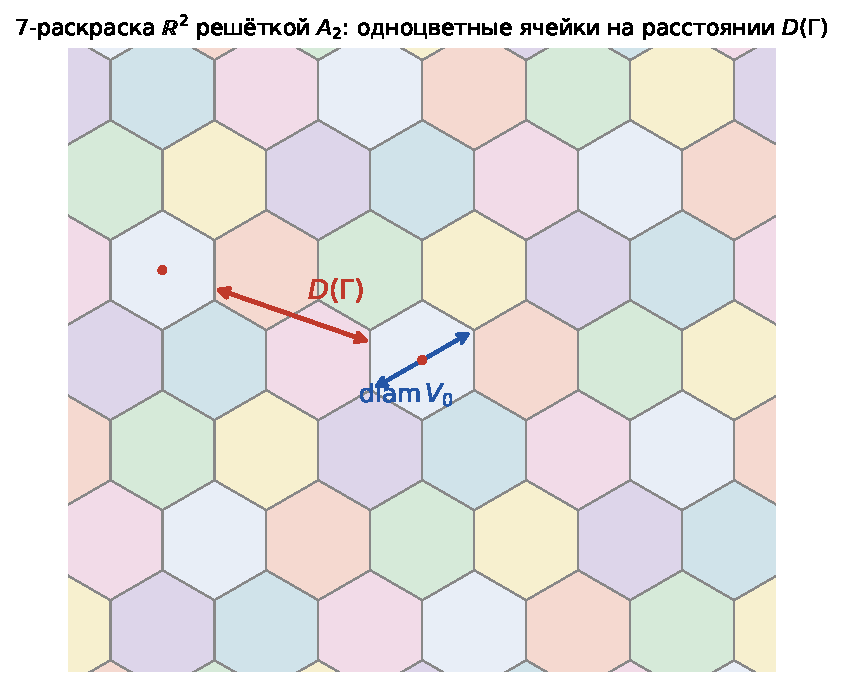
\includegraphics[width=0.66\textwidth]{fig_method.pdf}
\caption{Идея метода на примере $7$-раскраски плоскости шестиугольной решёткой
$A_2$ (классическая конструкция Исбелла, дающая $\chi(\R^2)\le7$). Каждая ячейка
Вороного (шестиугольник) окрашена цветом своего класса смежности по подрешётке
индекса~$7$; всего $7$ цветов. Две \emph{одноцветные} ячейки (красные точки)
разделены расстоянием $D(\Gamma)$, строго большим диаметра ячейки
$\diam V_0$. Раскраска запрещает все расстояния из промежутка
$\bigl(\diam V_0,\,D(\Gamma)\bigr)$.}
\label{fig:method}
\end{figure}

\subsection{Раскраска классами смежности}

Зафиксируем подрешётку $\Gamma\subseteq\Lambda$ индекса $k$ и окрасим каждую
ячейку $V_\Lambda(v)$ цветом класса смежности $v+\Gamma$. Так как классов ровно
$k$, получается $k$-цветная периодическая раскраска всего $\R^n$
(рис.~\ref{fig:method}). Ключевой вопрос: \emph{какие расстояния могут
разделять две одноцветные точки?}

Две точки одного цвета лежат либо в одной ячейке, либо в ячейках
$V_\Lambda(a)$, $V_\Lambda(b)$, центры которых отличаются на ненулевой вектор
$v=a-b\in\Gamma$. В первом случае расстояние не превосходит диаметра
$\diam V_0$; во втором --- не меньше расстояния между этими двумя ячейками.
Обозначим
\[
D(v)=\dist\bigl(V_0,\,v+V_0\bigr),\qquad
D(\Gamma)=\min_{v\in\Gamma\setminus\{0\}}D(v).
\]
Тогда множество \emph{реализуемых} одноцветных расстояний целиком лежит в
\[
[0,\ \diam V_0]\ \cup\ [D(\Gamma),\ \infty),
\]
а открытый промежуток $\bigl(\diam V_0,\,D(\Gamma)\bigr)$ \emph{свободен} ---
ни одна пара одноцветных точек не находится на таком расстоянии
(рис.~\ref{fig:interval}). Масштабируя решётку, этот свободный промежуток можно
совместить с любым наперёд заданным отрезком $[1,\ell]$, лишь бы отношение
\begin{equation}\label{eq:d-def}
d(\Lambda,\Gamma)\ :=\ \frac{D(\Gamma)}{\diam V_0}
\end{equation}
превосходило~$1$.

\begin{figure}[t]
\centering
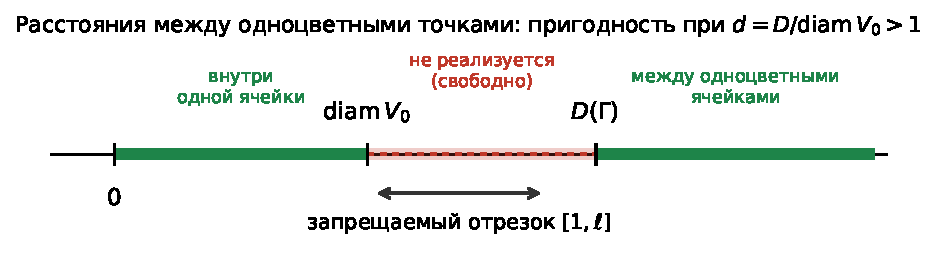
\includegraphics[width=0.86\textwidth]{fig_interval.pdf}
\caption{Расстояния между одноцветными точками (числовая ось). Реализуются лишь
малые (внутри одной ячейки, $\le\diam V_0$) и большие (между разными
одноцветными ячейками, $\ge D(\Gamma)$); промежуток между ними свободен. Если
$d=D(\Gamma)/\diam V_0>1$, то после нормировки $\diam V_0\mapsto{}$<<чуть меньше
$1$>> весь отрезок $[1,\ell]$ с $\ell<d$ попадает в свободную зону --- раскраска
правильна для $[1,\ell]$.}
\label{fig:interval}
\end{figure}

\begin{proposition}\label{prop:crit}
Если $d(\Lambda,\Gamma)>1$, то $\chi\bigl(\R^n,[1,\ell]\bigr)\le[\Lambda:\Gamma]$
при всех $\ell<d(\Lambda,\Gamma)$; в частности $\chi(\R^n)\le[\Lambda:\Gamma]$.
\end{proposition}
\begin{proof}
Возьмём масштаб $s>0$ с $s\,\diam V_0<1$ и $s\,D(\Gamma)>\ell$ --- это возможно
тогда и только тогда, когда $\ell<D(\Gamma)/\diam V_0=d$. Для решётки $s\Lambda$
свободный промежуток $\bigl(s\diam V_0,\,sD(\Gamma)\bigr)$ содержит весь отрезок
$[1,\ell]$, значит раскраска правильна для $[1,\ell]$. Случай $\ell=1$ (с учётом
\eqref{eq:mono}) даёт $\chi(\R^n)\le k$.
\end{proof}

Таким образом, вся задача сводится к поиску пары <<решётка + подрешётка>> с
возможно большим отношением~\eqref{eq:d-def}. Величину $d$ будем называть
\emph{нормированной шириной} (запрещённого интервала); чем она больше при данном
числе цветов $k$, тем сильнее оценка.

\subsection{Как считать $D(v)$: лемма о середине}

Прямое вычисление расстояния между двумя многогранниками --- задача негладкой
оптимизации. В~\cite{Ivanov2011} она сведена к расстоянию \emph{от точки до
одного многогранника} с помощью центральной симметрии ячеек Вороного
(классическое свойство, восходящее к Вороному \cite{Voronoi}).

\begin{lemma}[Вороной]\label{lem:sym}
Ячейка $V_0$ --- выпуклый центрально-симметричный многогранник, и все её грани
центрально-симметричны.
\end{lemma}

\begin{lemma}[о середине; {\cite[лемма~2]{Ivanov2011}}]\label{lem:mid}
Минимальное расстояние между ячейками $V_0$ и $v+V_0$ реализуется на паре
точек, симметричных относительно середины $v/2$ отрезка их центров. Как
следствие,
\begin{equation}\label{eq:mid}
D(v)=2\,\dist\bigl(v/2,\,V_0\bigr).
\end{equation}
\end{lemma}
\begin{proof}[Идея]
Пусть минимум достигается на $x\in V_0$, $y\in v+V_0$. Отражение через $v/2$
переводит (в силу леммы~\ref{lem:sym}) $V_0$ в $v+V_0$ и наоборот; образы
$x',y'$ дают ту же длину $|x'-y'|=|x-y|$. Середины отрезков $[x,y']$ и $[y,x']$
по выпуклости лежат в соответствующих ячейках, симметричны относительно $v/2$ и
реализуют то же минимальное расстояние. Значит, минимум достигается на
симметричной паре, а расстояние от каждой точки до $v/2$ равно $\dist(v/2,V_0)$.
\end{proof}

Формула~\eqref{eq:mid} превращает вычисление $D(v)$ в стандартную задачу
<<расстояние от точки до выпуклого многогранника>>.

\subsection{Полнота перебора соседей}

Минимум $D(\Gamma)=\min_v D(v)$ берётся по бесконечной подрешётке, но
перебирать нужно лишь \emph{конечное} множество коротких векторов. Так как
$V_0$ содержится в шаре радиуса $\tfrac12\diam V_0$, справедлива нижняя оценка
$D(v)\ge\|v\|-\diam V_0$. Поэтому если уже найден некоторый вектор с $D=D_{*}$,
то улучшить минимум могут только векторы с
\begin{equation}\label{eq:window}
\|v\|\ <\ D_{*}+\diam V_0.
\end{equation}
Это \emph{доказуемо полная} граница перебора (в отличие от эвристических
<<окон>>): она справедлива при любом базисе подрешётки и гарантирует, что ни
один потенциально лучший сосед не пропущен.

Наименьшее число цветов среди раскрасок описанного вида --- то есть минимум
$[\Lambda:\Gamma]$ по всем решёткам $\Lambda$, подрешёткам $\Gamma$ и
масштабам --- принято обозначать $\chi_s\bigl(\R^n,[1,\ell]\bigr)$; очевидно,
$\chi\bigl(\R^n,[1,\ell]\bigr)\le\chi_s\bigl(\R^n,[1,\ell]\bigr)$. Все
известные верхние оценки в малых размерностях, включая полученные ниже, --- это
оценки на $\chi_s$.

\begin{remark}[о границах ячеек]\label{rem:halfopen}
Ячейки Вороного замкнуты и пересекаются по границам, поэтому <<окрасим каждую
ячейку>> само по себе не задаёт функцию на $\R^n$. Как обычно, мы фиксируем
полуоткрытую фундаментальную область: из каждой пары соседних ячеек общая грань
приписывается одной из них. Все оценки ниже от этого выбора не зависят, так как
диаметр полуоткрытой ячейки не превосходит $\diam V_0$, а расстояние между
разноимёнными ячейками не меньше $D(v)$.
\end{remark}


